% Table 1 and the CONSORT diagram.
% Standalone sheet of paper/tables/table1.tex (approved 2026-10-20) and the
% CONSORT diagram. Build with: pdflatex table1 (x2)
\documentclass[11pt]{article}
\usepackage[a4paper,margin=1.6cm,top=1.4cm,bottom=1.4cm]{geometry}
\usepackage[T1]{fontenc}
\usepackage[utf8]{inputenc}
\usepackage{tgpagella,mathpazo}
\usepackage[scaled=0.95]{helvet}
\usepackage{microtype}
\usepackage{amsmath}
\usepackage{booktabs,tabularx,multirow}
\usepackage{graphicx}
\usepackage[dvipsnames]{xcolor}
\usepackage{caption}
\usepackage{tikz}
\usetikzlibrary{arrows.meta,backgrounds,calc,decorations.pathreplacing,fit,matrix,positioning,shapes.geometric}
\usepackage[hidelinks]{hyperref}
\usepackage[nameinlink,capitalise]{cleveref}
% Shared manuscript and TikZ visual language for the OPERA paper.
% Keep colours and Helvetica-like figure typography synchronized with
% opera/visualization/style.py (Arial/Liberation Sans on render hosts).

\definecolor{OperaIndigo}{HTML}{2D3A8C}
\definecolor{OperaNavy}{HTML}{1A237E}
\definecolor{OperaPeriwinkle}{HTML}{5C7AEA}
\definecolor{OperaSlate}{HTML}{737D8C}
\definecolor{OperaTeal}{HTML}{408579}
\definecolor{OperaGreen}{HTML}{1B7A4A}
\definecolor{OperaSienna}{HTML}{B5451B}
\definecolor{OperaTerracotta}{HTML}{C16A58}
\definecolor{OperaOchre}{HTML}{B18B4D}
\definecolor{OperaLavender}{HTML}{8974AC}
\definecolor{OperaInk}{HTML}{17212B}
\definecolor{OperaInkSecondary}{HTML}{485463}
\definecolor{OperaInkMuted}{HTML}{657180}
\definecolor{OperaBorder}{HTML}{CBD2DA}
\definecolor{OperaGrid}{HTML}{E8ECF1}
\definecolor{OperaPaper}{HTML}{F7F8FA}

\tikzset{
  opera/.style={font=\sffamily\small, text=OperaInk},
  panel/.style={draw=none, fill=white, inner sep=0pt},
  softpanel/.style={
    rounded corners=0.8mm,
    draw=OperaGrid,
    line width=0.45pt,
    fill=OperaPaper,
    inner sep=2.4mm,
  },
  stage/.style={
    rounded corners=0.7mm,
    draw=OperaBorder,
    line width=0.6pt,
    fill=white,
    align=center,
    minimum height=8mm,
    inner xsep=3mm,
    inner ysep=1.8mm,
  },
  stageblue/.style={stage, draw=OperaIndigo!55, fill=OperaIndigo!7},
  stageteal/.style={stage, draw=OperaTeal!65, fill=OperaTeal!8},
  stagewarm/.style={stage, draw=OperaSienna!60, fill=OperaSienna!7},
  latent/.style={
    circle,
    draw=OperaIndigo!65,
    fill=OperaIndigo!9,
    line width=0.6pt,
    minimum size=6mm,
    inner sep=0pt,
    font=\sffamily\scriptsize\bfseries,
  },
  token/.style={
    rounded corners=0.7mm,
    draw=OperaBorder,
    fill=white,
    minimum width=6.2mm,
    minimum height=4.8mm,
    inner sep=0.5mm,
    font=\sffamily\tiny,
    align=center,
  },
  outcome/.style={
    rounded corners=1mm,
    draw=OperaTerracotta!70,
    fill=OperaTerracotta!9,
    minimum height=5.8mm,
    inner xsep=1.8mm,
    font=\sffamily\scriptsize,
    align=center,
  },
  flow/.style={
    -{Latex[length=2mm,width=1.2mm]},
    line width=0.75pt,
    draw=OperaInkSecondary,
  },
  flowblue/.style={flow, draw=OperaIndigo},
  flowteal/.style={flow, draw=OperaTeal},
  flowwarm/.style={flow, draw=OperaSienna},
  relation/.style={
    -{Latex[length=1.8mm,width=1.1mm]},
    line width=0.65pt,
    draw=OperaLavender,
    densely dashed,
  },
  captionnote/.style={
    font=\sffamily\fontsize{6.6}{7.5}\selectfont,
    text=OperaInkMuted,
    align=center,
  },
  labelsmall/.style={
    font=\sffamily\fontsize{7}{8}\selectfont,
    text=OperaInkSecondary,
    align=center,
  },
  heading/.style={
    font=\sffamily\fontsize{9}{10}\selectfont\bfseries,
    text=OperaInk,
    align=left,
  },
  panelletter/.style={font=\sffamily\bfseries\normalsize, text=OperaInk},
  divider/.style={draw=OperaBorder, line width=0.45pt},
  eyebrow/.style={font=\sffamily\fontsize{6.5}{7.5}\selectfont\bfseries,
    text=OperaIndigo, align=left},
}

\newcommand{\placeholder}[1]{\textcolor{OperaSienna}{\textbf{[#1]}}}
\pagestyle{empty}
% The footnote points to the paper's supplementary index table, not part of this sheet.
\newcommand{\indextableref}{table of prognostic indices}

\begin{document}
\renewcommand{\cref}[1]{\indextableref}
% Only the patient-count row below has been updated for the released supervised population.
% All other numeric rows remain historical layout values and MUST be re-exported before use.
\begin{table*}[t]
\centering
\caption{Baseline characteristics of the supervised first-line haematology analysis cohort. \placeholder{All characteristics except patient counts require re-export from the current release.}}
\label{tab:characteristics}
\footnotesize
\setlength{\tabcolsep}{4pt}
\begin{tabularx}{\textwidth}{@{}Xrrrr@{}}
\toprule
Characteristic & Overall & Training & Tuning & Held-out \\
\midrule
Patients, $n$ & 37,531 & 29,105 & 1,980 & 6,446 \\
Age, years, median (IQR) & 69.3 (59.7--77.1) & 68.7 (59.2--76.5) & 71.1 (61.1--78.4) & 71.7 (61.7--78.8) \\
Age $\geq$70 years, $n$ (\%) & 18,011 (48.1\%) & 13,431 (46.1\%) & 1,050 (53.4\%) & 3,530 (55.2\%) \\
Female, $n$ (\%) & 15,647 (41.8\%) & 12,199 (41.9\%) & 802 (40.8\%) & 2,646 (41.4\%) \\
Male, $n$ (\%) & 21,820 (58.2\%) & 16,909 (58.1\%) & 1,165 (59.2\%) & 3,746 (58.6\%) \\
Year of first-line treatment, median (IQR) & 2016 (2010--2021) & 2014 (2009--2018) & 2022 (2022--2022) & 2024 (2023--2025) \\
Observed follow-up, years, median (IQR) & 4.1 (1.4--8.6) & 5.8 (2.1--10.1) & 3.5 (3.2--3.8) & 1.3 (0.6--2.2) \\
\addlinespace
\multicolumn{5}{@{}l}{\sffamily\bfseries Disease groups, $n$ (\%)}\\
Amyloidosis & 47 (0.1\%) & 22 (0.1\%) & 7 (0.4\%) & 18 (0.3\%) \\
\textbf{Burkitt/lymphoblastic lymphoma} & 1,364 (3.6\%) & 1,075 (3.7\%) & 87 (4.4\%) & 202 (3.2\%) \\
\hspace*{1em}Burkitt lymphoma (BL) & 295 (0.8\%) & 238 (0.8\%) & 15 (0.8\%) & 42 (0.7\%) \\
\hspace*{1em}Lymphoblastic lymphoma (LBL) & 1,069 (2.9\%) & 837 (2.9\%) & 72 (3.7\%) & 160 (2.5\%) \\
\textbf{CLL/SLL} & 5,152 (13.8\%) & 4,092 (14.1\%) & 244 (12.4\%) & 816 (12.8\%) \\
\hspace*{1em}Chronic lymphocytic leukaemia (CLL) & 4,062 (10.8\%) & 3,220 (11.1\%) & 187 (9.5\%) & 655 (10.2\%) \\
\hspace*{1em}Small lymphocytic lymphoma (SLL) & 1,090 (2.9\%) & 872 (3.0\%) & 57 (2.9\%) & 161 (2.5\%) \\
\textbf{DLBCL and related aggressive B-cell lymphomas} & 10,408 (27.8\%) & 8,369 (28.8\%) & 505 (25.7\%) & 1,534 (24.0\%) \\
\hspace*{1em}Diffuse large B-cell lymphoma (DLBCL) & 9,951 (26.6\%) & 8,008 (27.5\%) & 481 (24.5\%) & 1,462 (22.9\%) \\
\hspace*{1em}Richter transformation (RT) & 192 (0.5\%) & 151 (0.5\%) & 14 (0.7\%) & 27 (0.4\%) \\
\hspace*{1em}Transformed follicular lymphoma & 265 (0.7\%) & 210 (0.7\%) & 10 (0.5\%) & 45 (0.7\%) \\
Hairy-cell leukaemia & 418 (1.1\%) & 293 (1.0\%) & 29 (1.5\%) & 96 (1.5\%) \\
Hodgkin lymphoma & 2,644 (7.1\%) & 2,080 (7.1\%) & 141 (7.2\%) & 423 (6.6\%) \\
\textbf{Indolent B-cell non-Hodgkin lymphoma} & 5,399 (14.4\%) & 3,895 (13.4\%) & 302 (15.4\%) & 1,202 (18.8\%) \\
\hspace*{1em}Follicular lymphoma (FL) & 2,932 (7.8\%) & 2,248 (7.7\%) & 150 (7.6\%) & 534 (8.4\%) \\
\hspace*{1em}B-cell lymphoma, unspecified (BCL) & 227 (0.6\%) & 87 (0.3\%) & 17 (0.9\%) & 123 (1.9\%) \\
\hspace*{1em}Lymphoplasmacytic lymphoma (LPL) & 1,570 (4.2\%) & 1,165 (4.0\%) & 100 (5.1\%) & 305 (4.8\%) \\
\hspace*{1em}Extranodal marginal-zone lymphoma (EMZL) & 500 (1.3\%) & 318 (1.1\%) & 33 (1.7\%) & 149 (2.3\%) \\
\hspace*{1em}Nodal marginal-zone lymphoma (NMZL) & 27 (0.1\%) & 5 (0.0\%) & $<$5 & 22 (0.3\%) \\
\hspace*{1em}Splenic marginal-zone lymphoma (SMZL) & 143 (0.4\%) & 72 (0.2\%) & $<$5 & 69 (1.1\%) \\
Mantle-cell lymphoma & 1,466 (3.9\%) & 1,116 (3.8\%) & 87 (4.4\%) & 263 (4.1\%) \\
\textbf{Myeloma and related plasma-cell disorders} & 8,953 (23.9\%) & 6,904 (23.7\%) & 491 (25.0\%) & 1,558 (24.4\%) \\
\hspace*{1em}Multiple myeloma (MM) & 8,629 (23.0\%) & 6,673 (22.9\%) & 464 (23.6\%) & 1,492 (23.3\%) \\
\hspace*{1em}Plasma-cell leukaemia (PCL) & 201 (0.5\%) & 146 (0.5\%) & 18 (0.9\%) & 37 (0.6\%) \\
\hspace*{1em}Solitary myeloma/plasmacytoma & 123 (0.3\%) & 85 (0.3\%) & 9 (0.5\%) & 29 (0.5\%) \\
\textbf{T-cell non-Hodgkin lymphoma} & 1,616 (4.3\%) & 1,262 (4.3\%) & 74 (3.8\%) & 280 (4.4\%) \\
\hspace*{1em}Angioimmunoblastic T-cell lymphoma (AITL) & 483 (1.3\%) & 351 (1.2\%) & 26 (1.3\%) & 106 (1.7\%) \\
\hspace*{1em}Anaplastic large-cell lymphoma (ALCL) & 410 (1.1\%) & 339 (1.2\%) & 12 (0.6\%) & 59 (0.9\%) \\
\hspace*{1em}Peripheral T-cell lymphoma (PTCL) & 522 (1.4\%) & 444 (1.5\%) & 17 (0.9\%) & 61 (1.0\%) \\
\hspace*{1em}T-cell lymphoma, unspecified (TCL) & 201 (0.5\%) & 128 (0.4\%) & 19 (1.0\%) & 54 (0.8\%) \\
\addlinespace
\multicolumn{5}{@{}l}{\sffamily\bfseries Recorded performance status, $n$ (\%)}\\
Performance status 0 & 14,662 (53.8\%) & 11,842 (53.2\%) & 858 (54.3\%) & 1,962 (57.9\%) \\
Performance status 1 & 8,262 (30.3\%) & 6,838 (30.7\%) & 434 (27.5\%) & 990 (29.2\%) \\
Performance status 2 & 2,557 (9.4\%) & 2,077 (9.3\%) & 187 (11.8\%) & 293 (8.6\%) \\
Performance status 3 & 1,273 (4.7\%) & 1,063 (4.8\%) & 88 (5.6\%) & 122 (3.6\%) \\
Performance status 4 & 481 (1.8\%) & 444 (2.0\%) & 13 (0.8\%) & 24 (0.7\%) \\
Missing performance status$^{a}$ & 10,232 (27.3\%) & 6,844 (23.5\%) & 387 (19.7\%) & 3,001 (46.9\%) \\
\addlinespace
\multicolumn{5}{@{}l}{\sffamily\bfseries Disease-specific prognostic risk category, $n$ (\%)}\\
Low & 3,989 (17.6\%) & 3,231 (17.4\%) & 243 (17.6\%) & 515 (18.9\%) \\
Intermediate & 10,513 (46.4\%) & 8,608 (46.4\%) & 639 (46.3\%) & 1,266 (46.5\%) \\
High / very high$^{b}$ & 8,161 (36.0\%) & 6,721 (36.2\%) & 497 (36.0\%) & 943 (34.6\%) \\
Missing risk category$^{a}$ & 14,804 (39.5\%) & 10,548 (36.2\%) & 588 (29.9\%) & 3,668 (57.4\%) \\
\addlinespace
\multicolumn{5}{@{}l}{\sffamily\bfseries Pre-treatment record summaries, median (IQR)$^{c}$}\\
Recorded clinical-history span, years & \placeholder{Re-export} & \placeholder{Re-export} & \placeholder{Re-export} & \placeholder{Re-export} \\
Clinical-coded records & \placeholder{Re-export} & \placeholder{Re-export} & \placeholder{Re-export} & \placeholder{Re-export} \\
Distinct diagnosis codes & 21.0 (13.0--32.0) & 20.0 (12.0--30.0) & 24.0 (15.0--37.0) & 25.0 (15.0--38.0) \\
Distinct medication codes & 21.0 (12.0--34.0) & 18.0 (10.0--30.0) & 32.0 (21.0--46.0) & 34.0 (22.0--49.0) \\
Laboratory-coded records & 197.0 (0.0--482.0) & 118.0 (0.0--346.0) & 483.0 (279.5--803.5) & 531.0 (302.0--887.0) \\
\bottomrule
\end{tabularx}
\vspace{1.5mm}
\begin{minipage}{\textwidth}\scriptsize
One record per patient in the historical 37,467-person review export; these values are not the current 37,557-person first-line source or its supervised analysis subset. Disease groups are from \texttt{cohort\_grouped}, not the separate, incomplete \texttt{Disease} field. Indented rows show fine cohorts within their grouped parent; one-to-one groups are shown once. Disease percentages use the full cohort/split, not the parent group. A dash denotes an absent row in the source export, not a confirmed zero. Detailed treatment categories and scoring systems are reported in the supplementary tables.
$^{a}$Performance status and disease-specific prognostic risk categories are sourced from quality registries, whose disease and calendar-period coverage is incomplete. Category percentages use patients with nonmissing values; missingness percentages use the full cohort/split. The later-period decline in availability must be re-estimated from the current release before interpretation.
$^{b}$High and very high are combined only for this descriptive overview. The very-high category occurs in CLL-IPI (114 patients overall); risk categories from different scoring systems are not equivalent clinical scales. Original categories and scoring-system identities are retained in the supplement.
$^{c}$MEDS-derived values are provisional pending re-export after excluding demographic tokens from clinical-history summaries. Laboratory entries count coded records, not unique tests or verified source measurements. Follow-up is observed duration, not a reverse-Kaplan--Meier estimate.
IQR, interquartile range. Primary-only small-cell masking in the source exports is not disclosure clearance; the complete publication bundle requires institutional review.
\end{minipage}
\end{table*}

\clearpage
\begin{figure}[p]
\centering
\resizebox{!}{0.84\textheight}{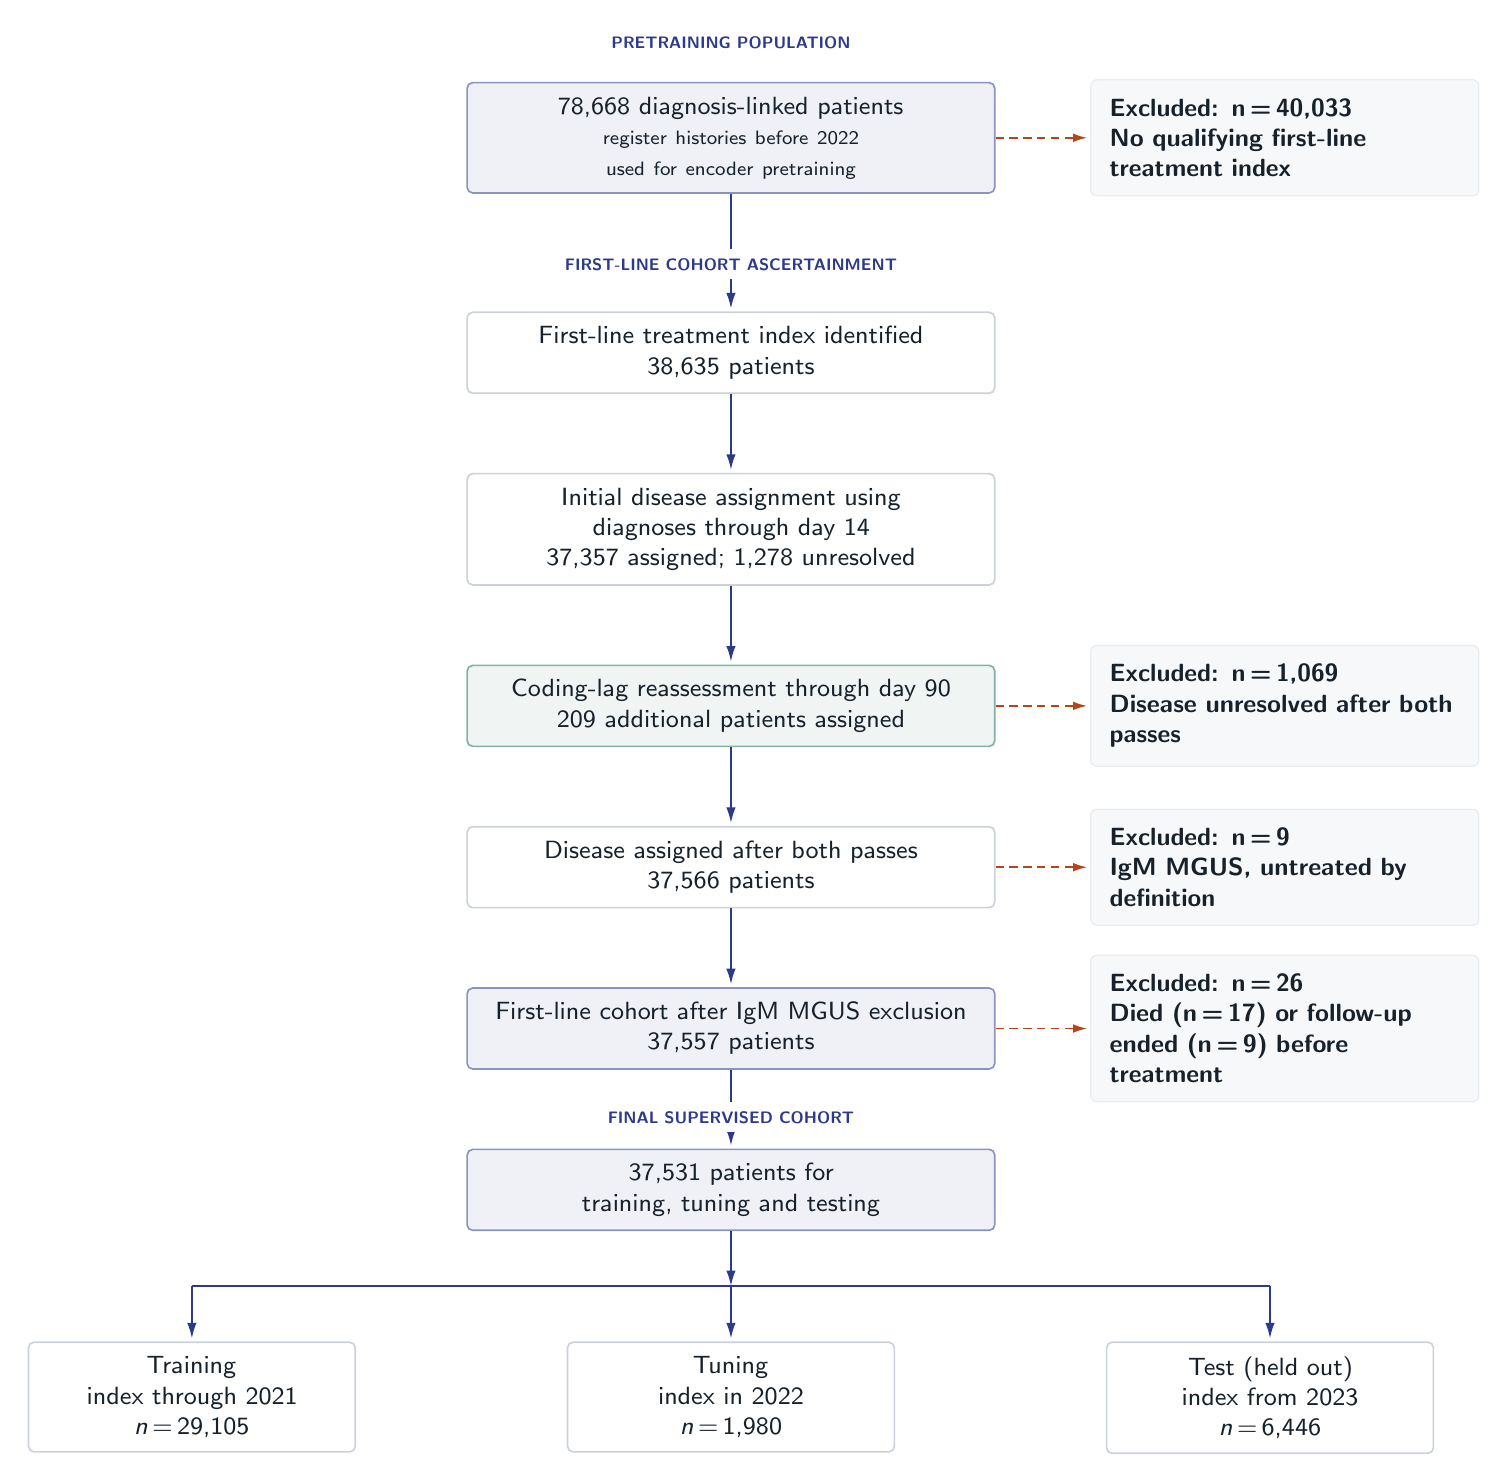
\begin{tikzpicture}[opera,node distance=10mm and 12mm,
    every node/.append style={execute at begin node={\hyphenpenalty=10000\exhyphenpenalty=10000}}]
  \node[stageblue,text width=6.1cm] (pretrainbox)
    {78,668 diagnosis-linked patients\\{\scriptsize register histories before 2022 used for encoder pretraining}};
  \node[eyebrow,above=3mm of pretrainbox] (pretrainlabel) {PRETRAINING POPULATION};
  \node[eyebrow,below=7mm of pretrainbox] (branchlabel)
    {FIRST-LINE COHORT ASCERTAINMENT};
  \node[stage,text width=6.1cm,below=4mm of branchlabel] (index)
    {First-line treatment index identified\\38,635 patients};
  \node[stage,text width=6.1cm,below=of index] (pass1)
    {Initial disease assignment using diagnoses through day 14\\37,357 assigned; 1,278 unresolved};
  \node[stageteal,text width=6.1cm,below=of pass1] (pass2)
    {Coding-lag reassessment through day 90\\209 additional patients assigned};
  \node[stage,text width=6.1cm,below=of pass2] (classified)
    {Disease assigned after both passes\\37,566 patients};
  \node[stageblue,text width=6.1cm,below=of classified] (firstline)
    {First-line cohort after IgM MGUS exclusion\\37,557 patients};
  \node[stageblue,text width=6.1cm,below=of firstline] (supervised)
    {37,531 patients for training, tuning and testing};

  \foreach \a/\b in {index/pass1,pass1/pass2,
                       pass2/classified,classified/firstline,firstline/supervised}
    \draw[flowblue,shorten >=1pt] (\a.south) -- (\b.north);
  \draw[flowblue,shorten >=1pt] (pretrainbox.south) -- (index.north);
  \node[eyebrow,fill=white,inner xsep=2mm] at (branchlabel) {FIRST-LINE COHORT ASCERTAINMENT};
  \node[eyebrow,fill=white,inner xsep=2mm,above=2mm of supervised]
    {FINAL SUPERVISED COHORT};

  % Mutually distinct exits from the central first-line flow.
  \node[softpanel,text width=4.45cm,align=left,right=of pretrainbox] (noindex)
    {\bfseries Excluded: \textit{n}\,=\,40{,}033\\No qualifying first-line treatment index};
  \node[softpanel,text width=4.45cm,align=left,right=of pass2] (unresolved)
    {\bfseries Excluded: \textit{n}\,=\,1{,}069\\Disease unresolved after both passes};
  \node[softpanel,text width=4.45cm,align=left,right=of classified] (secondary)
    {\bfseries Excluded: \textit{n}\,=\,9\\IgM MGUS, untreated by definition};
  \node[softpanel,text width=4.45cm,align=left,right=of firstline] (nosurvival)
    {\bfseries Excluded: \textit{n}\,=\,26\\Died (\textit{n}\,=\,17) or follow-up ended (\textit{n}\,=\,9) before treatment};
  \draw[relation,draw=OperaSienna,shorten >=1pt] (pretrainbox.east) -- (noindex.west);
  \draw[relation,draw=OperaSienna,shorten >=1pt] (pass2.east) -- (unresolved.west);
  \draw[relation,draw=OperaSienna,shorten >=1pt] (classified.east) -- (secondary.west);
  \draw[relation,draw=OperaSienna,shorten >=1pt] (firstline.east) -- (nosurvival.west);

  \node[stage,text width=3.55cm,below left=14mm and 14mm of supervised] (train)
    {Training\\index through 2021\\\textit{n}\,=\,29{,}105};
  \node[stage,text width=3.55cm,below=14mm of supervised] (tune)
    {Tuning\\index in 2022\\\textit{n}\,=\,1{,}980};
  \node[stage,text width=3.55cm,below right=14mm and 14mm of supervised] (held)
    {Test (held out)\\index from 2023\\\textit{n}\,=\,6{,}446};
  \coordinate (split) at ($(supervised.south)+(0,-7mm)$);
  \draw[flowblue] (supervised.south) -- (split);
  \draw[draw=OperaIndigo,line width=0.75pt]
    (train.north |- split) -- (held.north |- split);
  \foreach \dest in {train,tune,held}
    \draw[flowblue,shorten >=1pt] (\dest.north |- split) -- (\dest.north);

\end{tikzpicture}
}
\caption{\textbf{CONSORT diagram.} From the pretraining population, every DALY-CARE
patient with a lymphoid cancer or precursor (MGUS, MBL) diagnosis, to the final cohort and its temporal
split. A diagnosis was assigned to 37,357 patients from diagnoses recorded up to
14 days after treatment start, and to a further 209 on reassessment up to day 90
for late-coded diagnoses. Not every patient contributes to
every endpoint: outcome-specific eligibility, competing events and follow-up are
applied within each split.}
\label{fig:consort}
\end{figure}
\end{document}
